\chapter{Results and discussion}
\section{Data collection}
\label{results:collection}
Brazil, Mexico and India have been chosen for this experiment as Tinder is very
popular in these countries \citep{tinderPopular} and have much smaller
proportions of immigrant population compared to other countries in which Tinder
is popular such as the United States and the United Kingdom
\citep{desa2013trends}.

Using the state-of-art race recognition algorithms faces from Brazil and Mexico
would be classified as Hispanic so it would be interesting to see how well it
is possible to split this single class further. 

A non-capital city was chosen in each of the three countries and the data
collection service was tasked with setting its own location to those cities one
at a time and collecting pictures from local profiles for several days. The
breakdown of images collected per gender and location is summarised in
\Cref{table:results:dc:total_images}.
\begin{table}[t]
    \begin{center}
        \begin{tabular}{ c c c c c }
            \toprule
            Country       & City              & Male   & Female & Total \\ 
            \toprule
            Brazil  & Belo Horizonte &  4090 & 9688 & 13778\\
            India   & Mumbai         &  5014 & 3607 & 8621 \\
            Mexico  & Guadalajara    &  4887 & 3861 & 8748\\
            \bottomrule
        \end{tabular}
    \end{center}
    \caption{Total images collected by location and gender}
    \label{table:results:dc:total_images}
\end{table}

\section{Face and landmark detection}
\label{results:fd}
Images collected in the previous stage were passed through the face detection
stage to determine the presence of one or more faces and estimate the locations
of key facial landmarks. On average, the algorithm took around $6.5$ seconds to
perform face detection in a single image. Due to this limitation it was not
possible to detect faces in all images collected, however it was ensured that
at least 3000 images per location and gender passed through the face detection
stage. The actual numbers of images in which face detection was attempted can
be seen in \Cref{table:results:fd:detected}.
\begin{table}[t]
    \begin{center}
        \begin{tabular}{ c c c c}
            \toprule
            Country       & City              & Male   & Female\\ 
            \toprule
            Brazil  & Belo Horizonte &  3303 (81\%) & 6193 (64\%)\\
            India   & Mumbai         &  3771 (75\%) & 3149 (87\%)\\
            Mexico  & Guadalajara    &  3230 (66\%) & 3650 (95\%)\\
            \bottomrule
        \end{tabular}
    \end{center}
    \caption{Numbers and percentages of images passed through the face
    detection stage. Images in which there were no faces detected also
contribute to the numbers.}
    \label{table:results:fd:detected}
\end{table}

Every face detection has a score which determines how good the detection is.
\Cref{fig:results:fd:scores_hist} shows how the detection scores are
distributed relative to other classes.

\begin{figure}
    \centering
    \begin{subfigure}[b]{0.49\textwidth}
      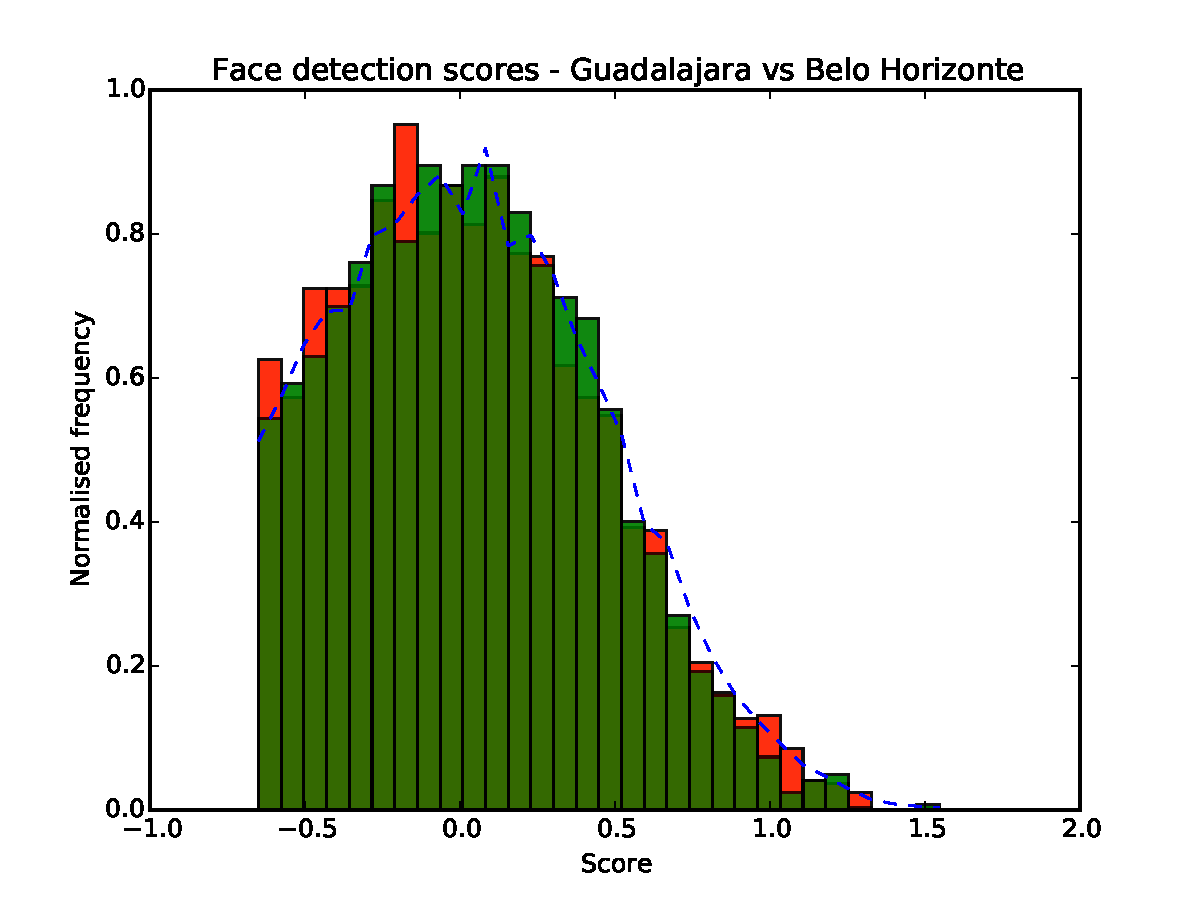
\includegraphics[width=\textwidth]{figures/results/scores_hist_Guadalajara_Belo_Horizonte}
      \caption{\textcolor{red}{Guadalajara} - \textcolor{green}{Belo Horizonte}}
    \end{subfigure}
    \begin{subfigure}[b]{0.49\textwidth}
      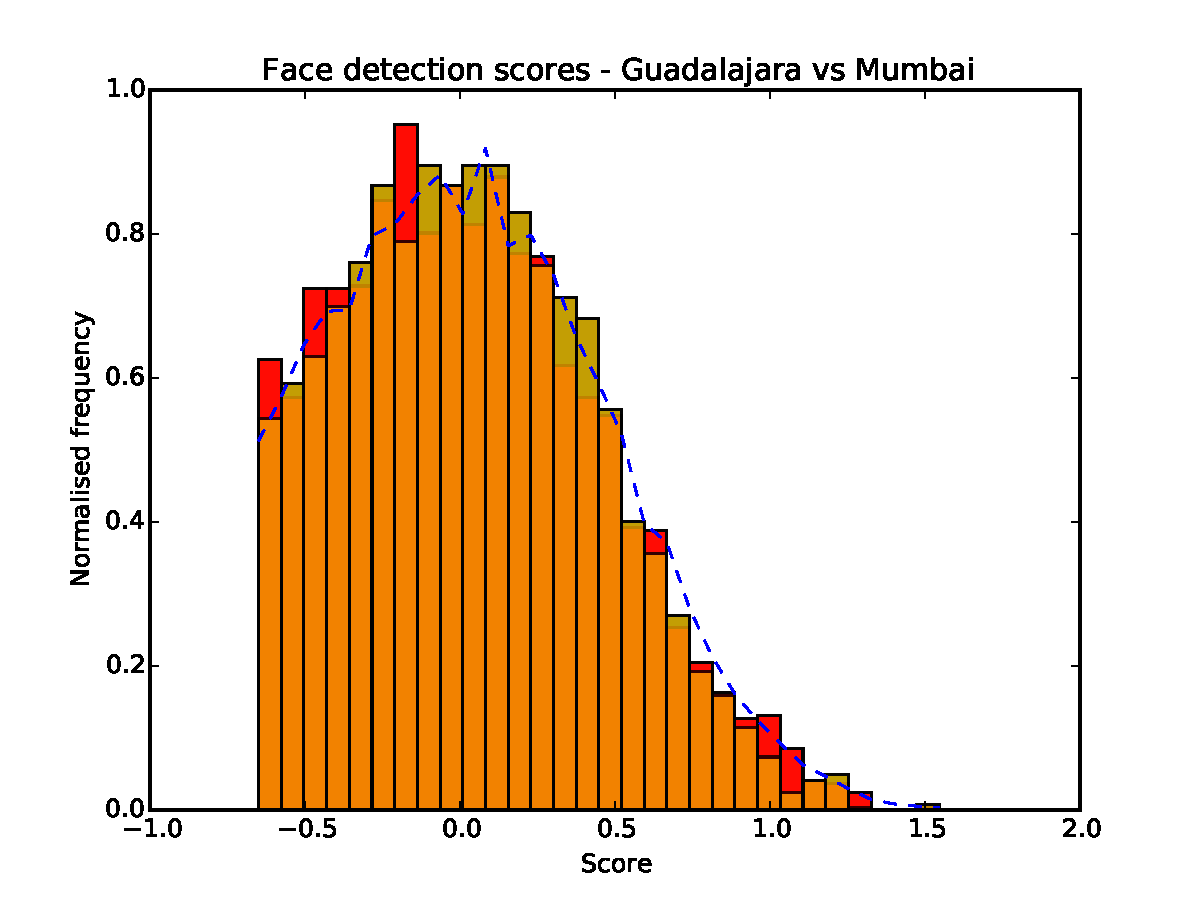
\includegraphics[width=\textwidth]{figures/results/scores_hist_Guadalajara_Mumbai}
      \caption{\textcolor{red}{Guadalajara} - \textcolor{orange}{Mumbai}}
    \end{subfigure}
    \begin{subfigure}[b]{0.49\textwidth}
      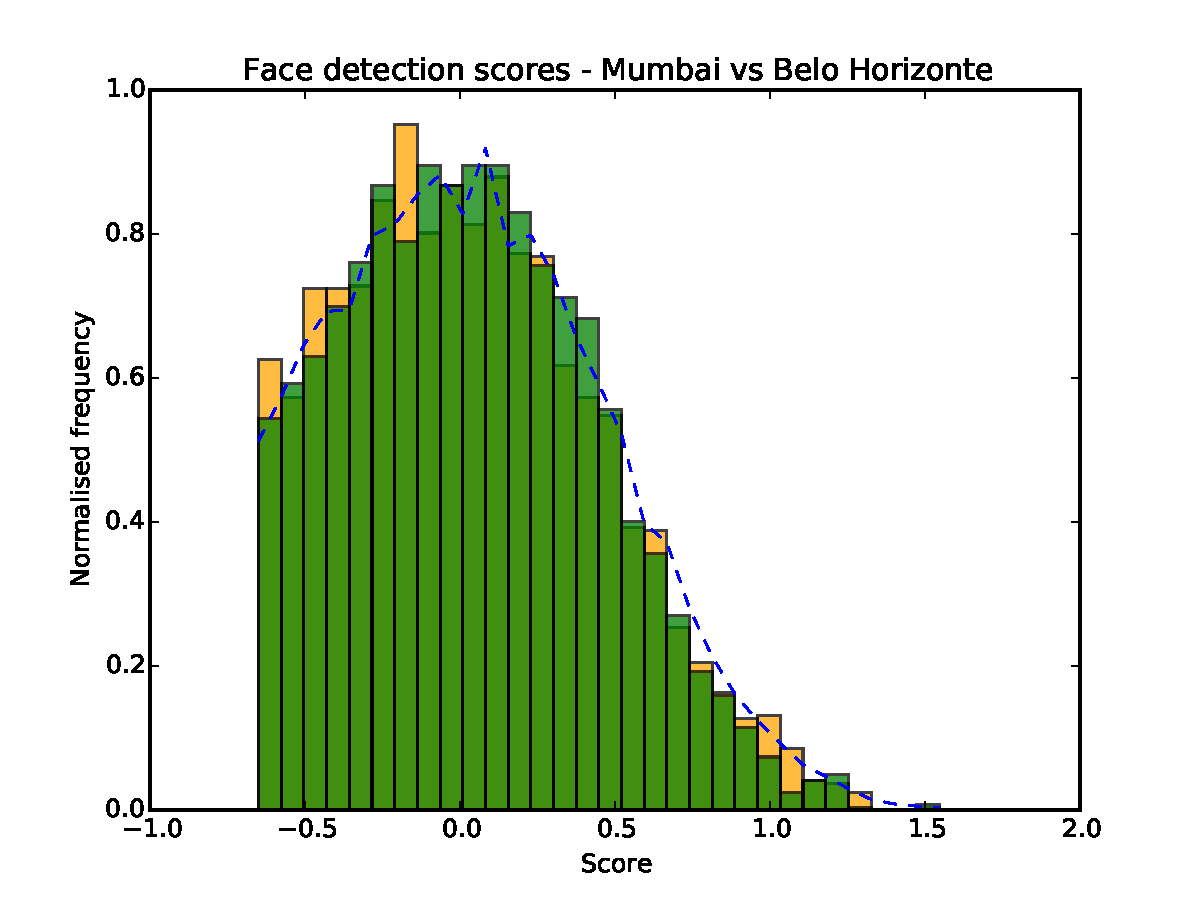
\includegraphics[width=\textwidth]{figures/results/scores_hist_Mumbai_Belo_Horizonte}
      \caption{\textcolor{orange}{Mumbai} - \textcolor{green}{Belo Horizonte}}
    \end{subfigure}
\caption{Normalised histograms of scores given by the face detection algorithm
to images from various locations. The blue dashed line represents the
normalised frequencies for all detections. Higher is better.}
\label{fig:results:fd:scores_hist}
\end{figure}

\Cref{fig:results:fd:good_detected} and \Cref{fig:results:fd:other_detected}
show examples of face detections with various scores.

\begin{figure}
    \centering
    \begin{subfigure}[b]{0.3\textwidth}
      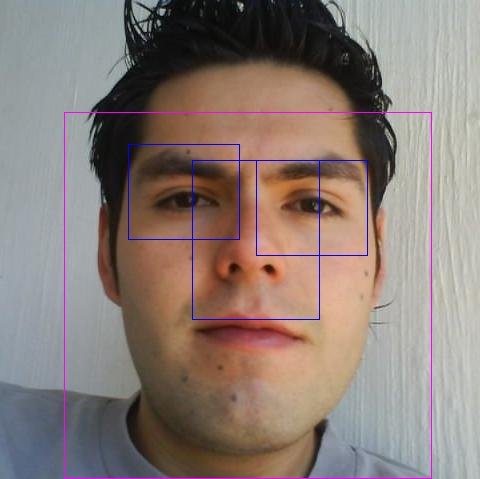
\includegraphics[width=\textwidth]{figures/results/detected_cff0618f-f631-4b0d-80d9-f582fee46fad}
      \caption{Score=1.4313}
      \label{fig:results:fd:good_detected1}
    \end{subfigure}
    \begin{subfigure}[b]{0.3\textwidth}
      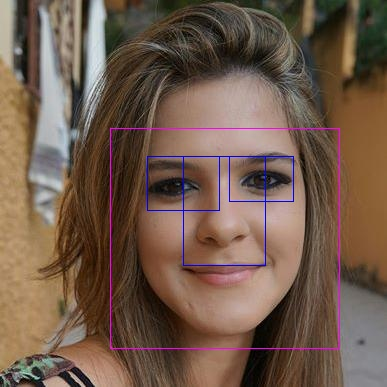
\includegraphics[width=\textwidth]{figures/results/detected_50508cb1-814e-4374-bf07-cef5c301c3c0}
      \caption{Score=1.20387}
      \label{fig:results:fd:good_detected2}
    \end{subfigure}
    \begin{subfigure}[b]{0.3\textwidth}
      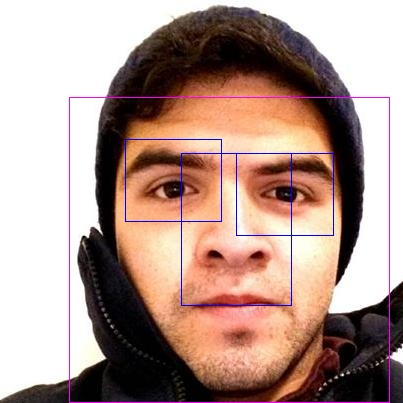
\includegraphics[width=\textwidth]{figures/results/detected_da153846-1afe-4b36-880a-bf8764bfd935}
      \caption{Score=1.09232}
      \label{fig:results:fd:good_detected3}
    \end{subfigure}
\caption{Three examples of high-scoring face detections.}
\label{fig:results:fd:good_detected}
\end{figure}

\begin{figure}
    \centering
    \begin{subfigure}[t]{0.3\textwidth}
      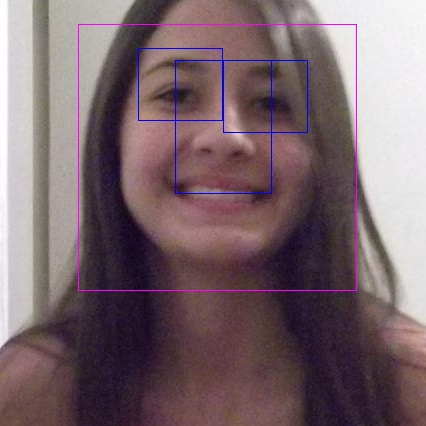
\includegraphics[width=\textwidth]{figures/results/detected_q3_15c3f02d-31c6-4955-8d05-c05029cdb473}
      \caption{Face detection with score=0.0651244 in upper quartile}
      \label{fig:results:fd:q3_detected2}
    \end{subfigure}
    \begin{subfigure}[t]{0.3\textwidth}
      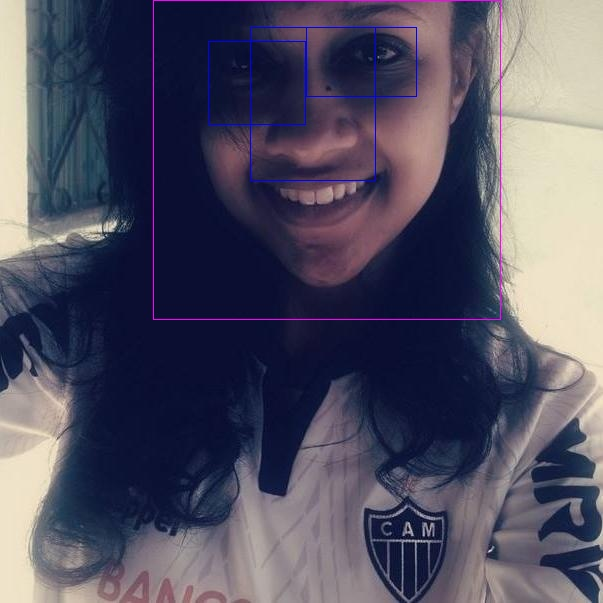
\includegraphics[width=\textwidth]{figures/results/detected_median_fcb1d3ed-7867-40ba-9691-8cd1f59dc36b}
      \caption{Face detection with score=-0.108765 around the median}
      \label{fig:results:fd:median_detected1}
    \end{subfigure}
    \begin{subfigure}[t]{0.3\textwidth}
      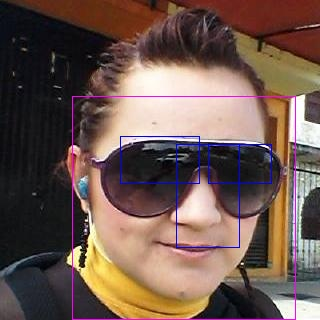
\includegraphics[width=\textwidth]{figures/results/detected_q1_f1c5f486-1697-4089-9bb6-7962d7db630c}
      \caption{Face detection with score=-0.517613 in lower quartile}
      \label{fig:results:fd:q1_detected3}
    \end{subfigure}
\caption{Examples of inferior face pictures. Cropped foreheads, blurriness,
sunglasses and small faces are some obvious reasons why a face detection might
have received a low score.}
\label{fig:results:fd:other_detected}
\end{figure}


\section{Data analysis and classification}
The data analysis software (\Cref{spec:analysis:software}) was designed and
implemented in such a way that the performance of different feature extraction
methods, classifiers and various parameters could be easily be compared by
creating separate configuration files for each setup.

The first attempt involved using Linear Discriminant Analysis (LDA) for feature
extraction and k-Nearest Neighbours to replicate the results from the most
similar study to this project - \citep{chinesegroups}. The average true
positive rate for this study was $0.7905$ across 3 classes.

Images had to undergo PCA transformation to reduce the their dimensions to $N -
c$ where $N$ is the number of training samples and $c$ is the number of
classes. This was required in order to make the covariance matrix full rank so
that it could be inverted when calculating the LDA weight vector.

Using the same approach as in this study resulted in rather poor classifier
performance as indicated in confusion matrices shown in
\Cref{table:results:ff_male_groups} and \Cref{table:results:ff_female_groups}.

\begin{table}[b]
      \centering
      \begin{tabular}{l c c c}
        \toprule
        &                    India(predicted)                 & Brazil(predicted)          & Mexico(predicted) \\
        \midrule
        India(actual)              &0.47&0.15&0.38\\  
        Brazil(actual)             &0.48&0.16&0.36\\ 
        Mexico(actual)             &0.44&0.15&0.41\\ 
        \addlinespace
      \end{tabular}
      \caption{PCA(d=N-c)+LDA and kNN(k=5): Male groups}
      \label{table:results:ff_male_groups}
\end{table}

\begin{table}[b]
  \centering
  \begin{tabular}{l c c c}
    \toprule
    &                    India(predicted)                 & Brazil(predicted)          & Mexico(predicted) \\
    \midrule
    India(actual)              &0.48&0.33&0.2 \\  
    Brazil(actual)             &0.46&0.36&0.18 \\ 
    Mexico(actual)             &0.4&0.28&0.32 \\  
    \addlinespace
  \end{tabular}
  \caption{PCA(d=N-c)+LDA and kNN(k=5): Female groups}
  \label{table:results:ff_female_groups}
\end{table}

The most likely reason for this is the lack of manually collected, high quality
dataset used in the \citep{chinesegroups} study. Experimenting with a wide
range of values for the number of dimensions used in PCA and LDA
transformations showed no significant change in classifier accuracy so this
approach was dismissed in favour of local binary patterns which proved to be
quite successful in a number of major-race classification studies
\citep{muhammadg}.

Using a support vector machine in combination with local binary patterns showed
consistent increase in classifier performance. The best SVM penalty parameter
$C$ was calculated to be $C=0.6$. The confusion matrices for male and female
subjects using this approach are shown in \Cref{table:results:best_male_groups}
and \Cref{table:results:best_female_groups}.

\begin{table}[b]
      \centering
      \begin{tabular}{l c c c}
        \toprule
        &                    India(predicted)                 & Brazil(predicted)          & Mexico(predicted) \\
        \midrule
        India(actual)              & 0.62                     & 0.18                       & 0.2 \\
        Brazil(actual)             & 0.2                      & 0.53                       & 0.27   \\
        Mexico(actual)             & 0.23                     & 0.31                       & 0.46 \\
        \addlinespace
      \end{tabular}
      \caption{LBP and SVM: Male groups}
      \label{table:results:best_male_groups}
    \end{table}

    \begin{table}[b]
      \centering
      \begin{tabular}{l c c c}
        \toprule
        &                    India(predicted)                 & Brazil(predicted)          & Mexico(predicted) \\
        \midrule
        India(actual)              & 0.67                     & 0.15                       & 0.18 \\
        Brazil(actual)             & 0.18                     & 0.59                       & 0.23   \\
        Mexico(actual)             & 0.2                      & 0.28                       & 0.52 \\
        \addlinespace
      \end{tabular}
      \caption{LBP and SVM: Female groups}
      \label{table:results:best_female_groups}
    \end{table}

These confusion matrices were calculated by selecting the top 600 faces for
each group as scored by the face detector. The 1800 images were randomly split
into training set (80\%) and test set (20\%), maintaining equal numbers of
samples in each class for each iteration of 6-fold cross validation. 


\subsection{Misclassified examples}
\begin{figure}
    \centering
    \begin{subfigure}[b]{0.3\textwidth}
      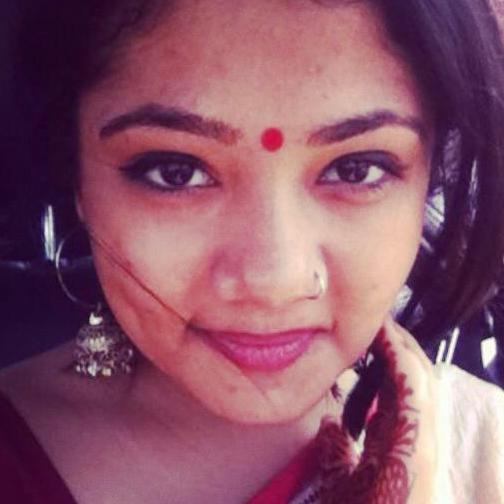
\includegraphics[width=\textwidth]{figures/results/misclassification/india-india.jpg}
      \caption{Correctly classified as Indian}
    \end{subfigure}
    \begin{subfigure}[b]{0.3\textwidth}
      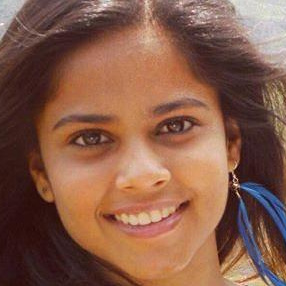
\includegraphics[width=\textwidth]{figures/results/misclassification/india-brazil.jpg}
      \caption{Misclassified as Brazilian}
    \end{subfigure}
    \begin{subfigure}[b]{0.3\textwidth}
      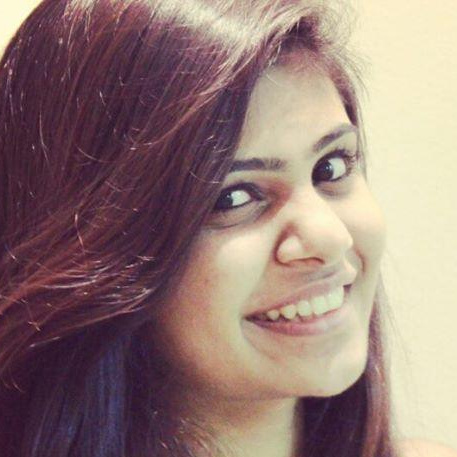
\includegraphics[width=\textwidth]{figures/results/misclassification/india-mexico.jpg}
      \caption{Misclassified as Mexican}
    \end{subfigure}
\caption{Correct and incorrect classifications of Indian subjects}
\label{fig:results:dc:misclass:india}
\end{figure}

\begin{figure}
    \centering
    \begin{subfigure}[b]{0.3\textwidth}
      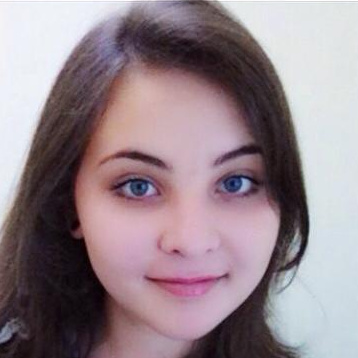
\includegraphics[width=\textwidth]{figures/results/misclassification/brazil-brazil.jpg}
      \caption{Correctly classified as Brazilian}
    \end{subfigure}
    \begin{subfigure}[b]{0.3\textwidth}
      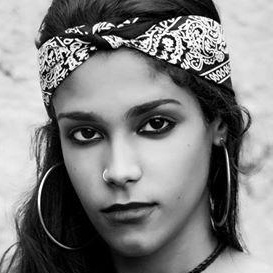
\includegraphics[width=\textwidth]{figures/results/misclassification/brazil-india.jpg}
      \caption{Misclassified as Indian}
    \end{subfigure}
    \begin{subfigure}[b]{0.3\textwidth}
        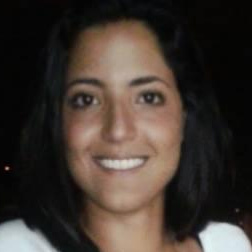
\includegraphics[width=\textwidth]{figures/results/misclassification/brazil-mexico.jpg}
      \caption{Misclassified as Mexican}
    \end{subfigure}
\caption{Correct and incorrect classifications of Brazilian subjects}
\label{fig:results:dc:misclass:brazil}
\end{figure}

\begin{figure}
    \centering
    \begin{subfigure}[b]{0.3\textwidth}
      
\includegraphics[width=\textwidth]{figures/results/misclassification/mexico-mexico.jpg}
      \caption{Correctly classified as Mexican}
    \end{subfigure}
    \begin{subfigure}[b]{0.3\textwidth}
      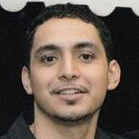
\includegraphics[width=\textwidth]{figures/results/misclassification/mexico-india.jpg}
      \caption{Misclassified as Indian}
    \end{subfigure}
    \begin{subfigure}[b]{0.3\textwidth}
        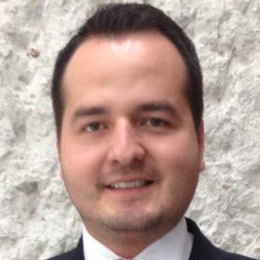
\includegraphics[width=\textwidth]{figures/results/misclassification/mexico-brazil.jpg}
      \caption{Misclassified as Brazilian}
    \end{subfigure}
\caption{Correct and incorrect classifications of Mexican subjects}
\label{fig:results:dc:misclass:mexico}
\end{figure}

\section{Conclusion}
The lack of the required data for this project was a hindrance and is the
reason for rather low classifier accuracy compared to the \citep{chinesegroups}
study, however this obstacle was used as motivation to explore the feasibility
of automatic data collection.

Images collected from a social network like Tinder come with an incredible
amount of noise and many additional steps are required to make this data as
useful as possible. In this project a face and landmark detector was used to
score images by their closeness to a series of predefined templates which
should match good pictures of human faces. The second stage of pre-processing
involved rotating, scaling and translating the images to ensure that most face
landmarks line up.

The accuracies achieved are within the expected range due given the quality of
the data and the difficult nature of determining one's location of origin. It
is impossible to come even close to 100\% accuracy as there is an incredible
number of possible classes considering how much different populations have
mixed in the history of humankind. 

\section{Future work}
Assigning classes like \textit{Indian} or \textit{Brazilian} is a simple
approach which will give us enough information, however it is flawed as it is
impossible to belong purely to a single race. A far better alternative would be
to give a list of possible locations from which a person is likely to originate
from. This list could be coupled with a list of probabilities to show the most
likely location first. This approach would work better with people of mixed
origin and in less ethnically homogeneous countries such as the United States.

Currently, the classifier requires different pre-trained models for male and
female subjects, however this requirement could be removed by incorporating a
gender recognition classifier.

\subsection{Pre-processing}
Computer-collected images have been adjusted for some landmark locations,
however the level of pre-process is by no means comprehensive and an additional
study may be required to assess a wider range of pre-processing methods. This
could include cropping faces by all landmarks appearing on the edges so that
the bounding area for rejecting the background is a polygon instead of a
rectangle. This approach would eliminate almost all background and thus
decrease noise in the data, potentially increasing classifier accuracy.


\subsection{Alternative features and classifiers}
The best method of feature extraction for this project was found to be local
binary patterns performed on the pre-processed image data, however it would
definitely be worth investigating if using a combination of other features
could improve classifier accuracy. There is a total of 68 landmarks detected in
each frontal face image which encode a substantial amount of new information
about images that otherwise would not be decoded using local binary patterns.

In the field of face recognition (recognising individual people) convolutional
networks are becoming increasingly more popular and achieve the highest
accuracies as measured by Area Under Curve (AUC) in the Labelled Faces in the
Wild (LFW) dataset benchmark \citep{LFWTechUpdate}. It may prove insightful to
explore the feasibility of using convolutional networks to solve the problem
discussed in this project as it may significantly improve classifier
performance. It would also be important to consider collecting significantly
more data than what is currently used.

\subsection{Implementation}
One of the biggest bottlenecks of the current pipeline (data collection
$\rightarrow$ face detection $\rightarrow$ classification) is the face detection
algorithm which takes $6.5$ seconds per image on average. The algorithm is
implemented in C++ and uses BLAS to perform various linear algebra computations
and after a thorough examination of the algorithm implementation there were no
obvious factors found which could contribute to its poor performance. It may be
useful to consider adapting some of its linear algebra operations to use
OpenCL.

The entire data analysis and classification suite is written in Python and
despite relying heavily on the highly optimised \texttt{numpy} package its
performance may be significantly improved by porting the current implementation
to C++, Julia or even Rust. The motivation for switching to a different
language originated in the process of implementing a parallel cross-validation
class which was problematic due to CPython's Global Interpreter Lock (GIL)
which severely reduces the speedup of using threads. 

%%% Local Variables: 
%%% mode: latex
%%% TeX-master: "thesis"
%%% End: 

